\documentclass{article}
\usepackage[english]{babel}
\usepackage[utf8]{inputenc}
\usepackage[affil-it]{authblk}
\usepackage{hyperref,tikz,times,pifont}
\usetikzlibrary{backgrounds,patterns,matrix,calc,decorations.pathreplacing,decorations.pathmorphing,arrows.meta,shadows,decorations.pathreplacing,positioning,shapes.misc}

%---------------------------------------------------------------------------------------------------------------------------
\definecolor{telecom}{RGB}{191,18,56}
\hypersetup{colorlinks=true, breaklinks=true, citecolor=telecom}
\newcommand{\cmark}{\textcolor{green}{\textbf{\ding{51}}}}
\newcommand{\xmark}{\textcolor{red}{\textbf{\ding{55}}}}	

\author{Bastien \textsc{Sultan}, Ludovic \textsc{Apvrille}
	\thanks{\{bastien.sultan, ludovic.apvrille\}@telecom-paris.fr}}
\affil{\emph{Télécom Paris}\\\emph{LabSoC Research Group}\\\emph{450, route des Chappes, F-06410 Biot}}
\title{\textbf{A tutorial on W-Sec}\\---\\A formal model-based method for assessing the impact of countermeasures}
\date{}

\begin{document}
\begin{figure}[t]
	\centering
	
\includegraphics[scale=.4]{figures/logo.pdf}
\end{figure}
\maketitle


%---------------------------------------------------------------------------------------------------------------------------
\section{Summary}

This document provides a tutorial on W-Sec, a method dedicated to quantify the (positive or negative) impacts of security countermeasures deployed on cyber-physical systems. The tutorial uses models of an autonomous swarm of rovers, designed in the context of the EU H2020 SPARTA project: the SPARTA deliverable~\cite{d51} describes in Sect.~2.1.2.2 the modeled rovers. In this case-study, a rover acts as a leader while the others act as followers: the leader periodically sends its speed values or emergency brake orders to the followers so that they can adapt their own speed consequently.

Both W-Sec and this autonomous rovers swarm case-study have been introduced in a paper presented at the 10\textsuperscript{th} Modelsward conference~\cite{wsec}.


\tableofcontents
\newpage


%---------------------------------------------------------------------------------------------------------------------------
\section{Getting started}

W-Sec relies on TTool and uses ProVerif~\cite{proverif} for security properties verification. Therefore, you should first install TTool and ProVerif.

\subsection{Installing TTool}

You will find here a tutorial on TTool installation: \url{https://ttool.telecom-paris.fr/installation.html}. To make sure you have the latest stable version, we recommend the \textbf{installation from the public Gitlab}.

\subsection{Installing ProVerif}

ProVerif can be downloaded and installed from this page: \url{https://bblanche.gitlabpages.inria.fr/proverif/}.

\subsection{Configuring TTool}

Once TTool and ProVerif have been installed, you can now configure your TTool version.
\begin{enumerate}
	\item In your TTool directory, open the configuration file (TTool/bin/config.xml).
	\item Modify the following line: \begin{verbatim}<ProVerifVerifierPath data="../../proverif"/>\end{verbatim} by replacing \texttt{../../proverif} with your ProVerif installation path.
\end{enumerate}



%---------------------------------------------------------------------------------------------------------------------------
\section{Prerequisiste}

Knowledge of TTool and AVATAR \& DIPLODOCUS SysML profiles should greatly facilitate your understanding of this tutorial. 
You can find an exhaustive documentation and tutorials on AVATAR in this page: \url{https://ttool.telecom-paris.fr/avatar.html}. 
This page contains links to videos on how to make a first model and how to simulate and verify a model.
In addition, you will find a complete tutorial on DIPLODOCUS by following this link: \url{https://ttool.telecom-paris.fr/docs/Tutorial.pdf}.



%---------------------------------------------------------------------------------------------------------------------------
\section{A quick overview of W-Sec}

\begin{figure}[t]
	\hspace*{-2cm}
	\centering
	\definecolor{tptred}{RGB}{191,18,56} 
\definecolor{tptbrown}{RGB}{109,80,71}
\begin{tikzpicture}[scale=.6, every node/.style={scale=.6}]
	\tikzstyle{avatarnode}=[rectangle,thick,draw,rounded corners=4pt,minimum width=2.5cm,text width=3.5cm,text centered,fill=white]
	\tikzstyle{avatar2ndnode}=[rectangle,thick,draw,rounded corners=4pt,minimum width=2.5cm,text width=3.5cm,text centered,fill=gray!40]
	\tikzstyle{assessment}=[chamfered rectangle,thick,draw,minimum width=2.5cm,text width=3.5cm,text centered,fill=gray!80]
	\tikzstyle{diplodocusnode}=[rectangle,thick,draw,rounded corners=4pt,minimum width=2.5cm,text width=3.5cm,text centered,fill=white]
	\tikzstyle{diplodocus2ndnode}=[rectangle,thick,draw,rounded corners=4pt,minimum width=2.5cm,text width=3.5cm,text centered,fill=gray!40]
	\tikzstyle{attackpatchnode}=[rectangle,thick,draw,minimum width=2.5cm,text width=3.5cm,text centered,fill=white]
	\tikzstyle{arrow}=[->,thick,rounded corners=4pt]
	\tikzstyle{arrowd}=[->,thick,decorate,decoration={snake,amplitude=1pt,segment length=1.5mm,post length=1mm}]
	\tikzstyle{arrowpv}=[->,thick,dashed,decorate,decoration={snake,amplitude=1.5pt,segment length=5mm,post length=1mm}]
	\tikzstyle{arrowsim}=[->,thick,dotted,decorate,decoration={snake,amplitude=1.5pt,segment length=5mm,post length=1mm}]
	\tikzstyle{arrowfeedback}=[->,thick,dotted,rounded corners=4pt]

	\node[diplodocusnode,copy shadow,fill=tptred!25] (diplodocus) at (0,0) {\large{Components models\\(\textbf{HW/SW partitioning})}};
	\node[attackpatchnode] (attackpatch) at (4.5,0) {\large{Attack scenarios + Countermeasures description}};
	\node[avatarnode,copy shadow,fill=tptbrown!25] (avatar) at (9,0) {\large{System model\\+ \emph{all test scenarios}\\(\textbf{High-level design})}};

	\node[diplodocus2ndnode,double copy shadow,fill=tptred!50] (diplodocusmutant) at (7.5,-10) {\large{Components models\\+ Attacks\\+ Countermeasures}};

	\node[assessment,fill=tptred!75] (diplodocusregression) at (15,1) {\large{Regression assessment\\(w.r.t. performance)}};
	\node[assessment,fill=tptred!75] (diplodocussecurity) at (15,-1) {\large{Security assessment}};


	\node[avatar2ndnode,double copy shadow,fill=tptbrown!50] (avatarpatched) at (15.75,-5) {\large{System model\\+ Countermeasures\\+ \emph{all test scenarios}}};
	\node[avatar2ndnode,double copy shadow,fill=tptbrown!50] (avatarattacked) at (15.75,-7.5) {\large{System model\\+ Attacks\\+ \emph{relevant test sc.}}};
	\node[avatar2ndnode,text opacity=0,fill=tptbrown!50] (avatarattackedpatchedshadow) at (16.15,-9.6) {\large{System model\\+ Attacks\\+ Countermeasures\\+ \emph{relevant test sc.}}};
	\node[avatar2ndnode,double copy shadow,fill=tptbrown!50] (avatarattackedpatched) at (15.75,-10) {\large{System model\\+ Attacks\\+ Countermeasures\\+ \emph{relevant test sc.}}};

	\node[assessment,fill=tptbrown!75] (avatarregression) at (22.5,1) {\large{Regression assessment\\(w.r.t. safety)}};
	\node[assessment,fill=tptbrown!75] (avatarefficiency) at (22.5,-1) {\large{Efficiency assessment\\(w.r.t. safety)}};



	\draw[arrow,color=tptbrown] (avatar.south) -- (avatarpatched.west);
	\draw[arrow,color=tptbrown] (avatar.south) -- (avatarattacked.west);
	\draw[arrow,color=tptbrown,shorten >=7pt] (avatarattacked.south) -- (avatarattackedpatched.north) ;

	\draw[->,thick,decorate,decoration={snake,amplitude=1pt,segment length=1.5mm,post length=1mm,pre length=4mm},shorten <=10pt,color=tptbrown] (avatarpatched.east) -- (avatarregression.west);
	\draw[->,thick,decorate,decoration={snake,amplitude=1pt,segment length=1.5mm,post length=1mm,pre length=4mm},shorten <=10pt,color=tptbrown] (avatarattacked.east) -- (avatarefficiency.west);
	\draw[->,thick,decorate,decoration={snake,amplitude=1pt,segment length=1.5mm,post length=1mm,pre length=7mm},shorten <=19pt,color=tptbrown] (avatarattackedpatched.east) -- (avatarefficiency.south west);



	
	\draw[arrow,color=tptred,shorten >=6pt] (diplodocus.south) -- (diplodocusmutant.north);
	\draw[->,thick,dotted,decorate,decoration={snake,amplitude=1.5pt,segment length=5mm,pre length=3mm,post length=1mm},shorten <=6pt,color=tptred] (diplodocusmutant.north) -- (diplodocusregression.west);
	\draw[->,thick,dashed,decorate,decoration={snake,amplitude=1.5pt,segment length=5mm,pre length=3mm,post length=1mm},shorten <=6pt,color=tptred] (diplodocusmutant.north) -- (diplodocussecurity.west);

	\node[align=left] (arrowcaption) at (1.8,-11.5) {\large{: Model mutation}};
	\node[align=left] (arrowsimcaption) at (4.05,-12) {\large{: Simulation (with TTool internal simulator)}};
	\node[align=left] (arrowpvcaption) at (14.66,-11.5) {\large{: Model-checking (with ProVerif)}};
	\node[align=left] (arrowdcaption) at (16.47,-12) {\large{: Model-checking (with TTool internal model-checker)}};
	\node[align=left] (arrowfeedbackcaption) at (6.42,-12.5) {\large{: Feedback to components, system, countermeasures and attacks models}};
	\draw[arrow] (-1.5,-11.5) -- (arrowcaption);
	\draw[arrowsim] (-1.5,-12) -- (arrowsimcaption);
	\draw[arrowpv] (10,-11.5) -- (arrowpvcaption);
	\draw[arrowd] (10,-12) -- (arrowdcaption);
	\draw[arrowfeedback] (-1.5,-12.5) -- (arrowfeedbackcaption);

	\draw[-,thick,dashed,shorten <=2pt] (diplodocus) -- (attackpatch);
	\draw[-,thick,dashed,shorten <=2pt] (avatar) -- (attackpatch);


	\draw[decorate,decoration={brace,raise=.25cm},thick] (diplodocusregression.north) -- (avatarregression.north)node[above,pos=.5,text width=10cm,text centered]{};
	\draw[arrowfeedback,shorten >=2pt] (18.75,2.4) -- (18.75,2.75) -| (avatar.north);
	\draw[arrowfeedback] (18.75,2.4) -- (18.75,3.25) -| (attackpatch.north);
	\draw[arrowfeedback,shorten >=2pt] (18.75,2.4) -- (18.75,3.75) -| (diplodocus.north);

	\begin{pgfonlayer}{background}
	\filldraw[color=gray!25,opacity=0.5] (diplodocusmutant.west) -- (diplodocusregression.west) -- (diplodocusregression.south east) -- (diplodocusmutant.south east);
	\filldraw[color=gray!12.5] (diplodocus.east) -- (diplodocusmutant.south east) -- (diplodocusmutant.south west) -- (diplodocus.south west) -- (diplodocus.west);
	\filldraw[color=gray!25,opacity=0.5] (avatar.east) -- (avatarpatched.north west) -- (avatarpatched.north) -- (avatarattackedpatched.south) -- (avatarattackedpatched.south west) -- (avatar.south west) -- (avatar.west);
	\filldraw[color=gray!12.5] (avatarpatched.north east) -- (avatarregression.west) -- (avatarregression.south east) -- (avatarattackedpatched.south east) -- (avatarattackedpatched.north) -- (avatarpatched.south);
	\end{pgfonlayer}


	\node[circle,thick,fill=white,draw] at (-2.5,0) {\huge{\textbf{1}}};
	\node[circle,thick,fill=white,draw] at (11.5,-7.5) {\huge{\textbf{2}}};
	\node[circle,thick,fill=white,draw] at (18.75,0) {\huge{\textbf{3}}};
	\node[circle,thick,fill=white,draw] at (11.5,3.25) {\huge{\textbf{4}}};

\end{tikzpicture}

	\caption{The W-Sec method (adapted from~\cite{wsec})}
	\label{fig:method}
\end{figure}

W-Sec is a four-stage method (see figure.~\ref{fig:method}). Its first stage is an \textbf{initial modeling stage}, where the system is modeled using the AVATAR and the DIPLODOCUS view:
\begin{itemize}
	\item The AVATAR view is used to model the system from a high-level architecture and behavior perspective.
	\item The DIPLODOCUS view is used to model the system's components\footnote{A \emph{component} is any equipment of the system, e.g. a network switch, a programmable logic controller, a computer, etc.} from a low-level hardware and software perspective. One DIPLODOCUS model is built per component we want to study.
\end{itemize}

Its second stage is a \textbf{mutation stage}, where the models are modified in order to enrich them with (i) the (safety and security) countermeasures we want to assess and (ii) the attack scenarios we want to protect the system from.

Its third stage is a \textbf{verification stage}, where we assess the impacts of the modeled countermeasures thanks to formal verification and simulation.

Last, its fourth stage is an \textbf{enrichment stage}, where the models of the system are enriched with the chosen countermeasure, if a countermeasure is finally chosen to be deployed.


%---------------------------------------------------------------------------------------------------------------------------
\section{W-Sec in Practice: modeling the system}

The first W-Sec stage is a modeling stage. As said previously, W-Sec uses two modeling views for these needs: the AVATAR view, and the DIPLODOCUS view.

\subsection{AVATAR view: a system-level modeling}

\subsubsection{The model}

The models designed in this view target capturing high-level architectural and behavioral (discrete and, if applicable, continuous) aspects of the system. The \textbf{wsec\_avatar.xml} file contains AVATAR models of the swarm: open this model in TTool and click on the tab ``\textbf{Nominal}''. You should now see the model depicted in figure~\ref{fig:avatarmodel}.

\begin{figure}
	\centering
	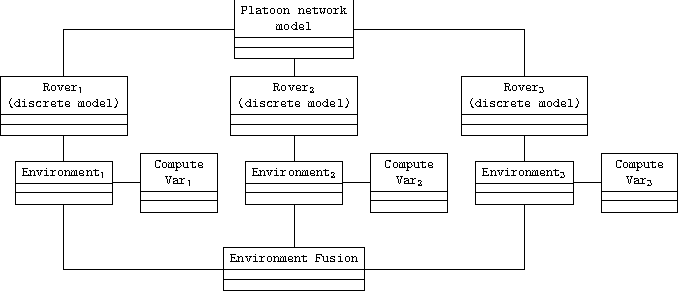
\includegraphics{figures/avatarmodel.pdf}
	\caption{System view of the swarm using AVATAR}
	\label{fig:avatarmodel}
\end{figure}

Here, each of the three rovers is modeled thanks to three blocks: \texttt{Rover$_i$} models its discrete behavior, while \texttt{Environment$_i$} and \texttt{ComputeVar$_i$} are two blocks modeling the continuous (dynamic) behavior of the rover. You should also see two yellow blocks: \texttt{Rover} and \texttt{Environment\_Library}. These blocks are \emph{libraries}, i.e. templates of blocks that can be instanciated in the AVATAR model. In our rover swarm model, \texttt{Rover$_1$}, \texttt{Rover$_2$} and \texttt{Rover$_3$} are instances of the \texttt{Rover} library, and \texttt{Environment$_1$}, \texttt{Environment$_2$} and \texttt{Environment$_3$} are instances of the \texttt{EnvironmentLibrary} library. \texttt{Network} block models the swarm's communication network, and \texttt{EnvironmentFusion} is a block used to disseminate the rovers coordinates among the different rovers dynamic models. In short, this model encompasses the whole system and its environment, i.e., the three rovers and their communication network.

\begin{figure}
	\centering
	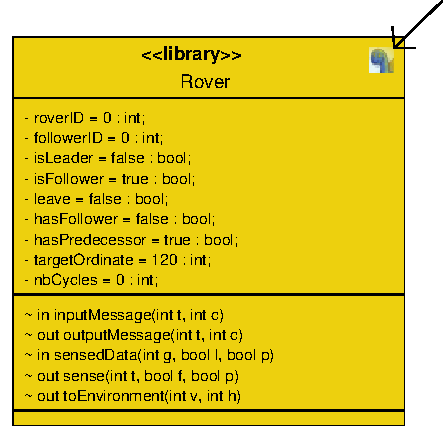
\includegraphics[scale=.6]{figures/roverlibrary.pdf}
	\caption{The \texttt{Rover} library}
	\label{fig:opensmd}
\end{figure}

Now, open the state machine diagram of the \texttt{Rover}'s $<<$library$>>$  by double-clicking on the blue turtle in the upper right corner of the block (see Figure~\ref{fig:opensmd}). Alternatively, you can open the state machine diagram either on clicking on its corresponding tab, or on selecting it in the main tree on the left of the TTool's window. 

In this state machine, the four states prefixed with the letter ``F'' model the discrete behavior of the rover when acting as a follower (see Figure~\ref{fig:roversmd}). This state machine diagram illustrates the modeling approach of the AVATAR view: we consider only the high-level behavior of the algorithms. Here, for instance, we don't model the computations of the PID controller used for speed control: we directly consider that the rover's speed is equal to the received setpoint.

\begin{figure}
	\centering
	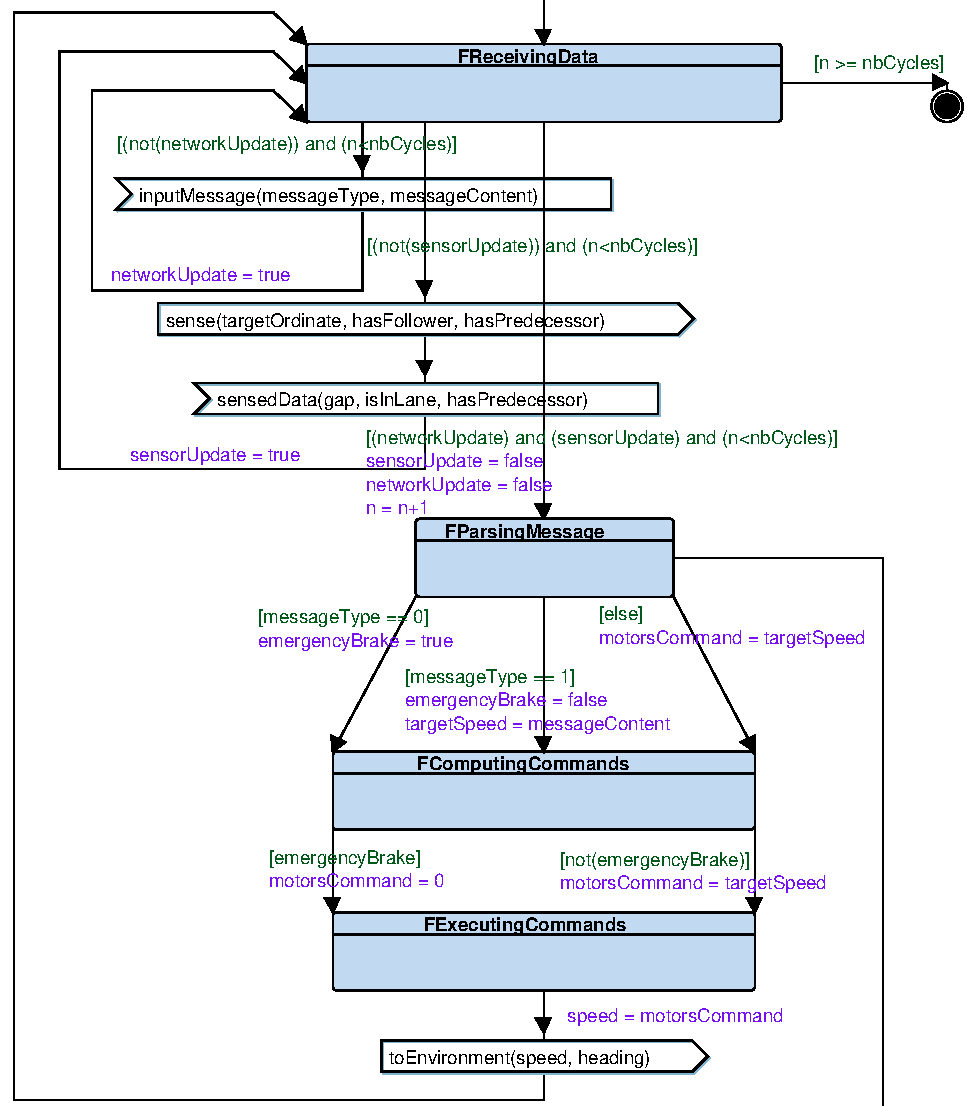
\includegraphics[scale=.6]{figures/roverfsm.pdf}
	\caption{Excerpt of the state machine diagram of the \texttt{Rover} $<<$library$>>$}
	\label{fig:roversmd}
\end{figure}

\subsubsection{Safety properties}

You should also notice, in the upper left corner of the Block Diagram, a pink box with two CTL* formulas:
\begin{verbatim}
A[] Environment2.gap>0
A[] Environment3.gap>0
\end{verbatim}
Indeed, in W-Sec, we verify the safety aspects in the AVATAR view: once the model has been designed in the modeling stage, we define the safety properties we want the system to comply with. Here, these two formulas express the following safety properties: (i) the gap ahead of rover$_2$ is always positive and (ii) the gap ahead of rover$_3$ is always positive. In other terms, we assume that these two properties are satisfied iff no crash occurs in the swarm. Note that we can express safety properties with CTL* formulas but also by right-clicking on the desired state in a state machine diagram and selecting ``check for reachability/liveness''.

\subsubsection{About functional scenarios}

You certainly have noticed that \textbf{wsec\_avatar.xml} has several tabs: for instance, \textbf{Nominal} and \textbf{Nominal\_Deceleration}. Indeed, we usually want to assess the countermeasures impacts according to different functional scenarios. Basically, two models capturing two different functional scenarios have slight variations (for instance, different initial values of a given variable, one additional state and several transitions in a state machine diagram, etc.). Therefore, we need several AVATAR models for modeling the different desired functional scenarios. Here, models correspond respectively to the following scenarios: (i) the leader runs at a constant speed and (ii) the leader decelerates.


\subsection{DIPLODOCUS view: a component-level modeling}

The DIPLODOCUS view is used for modeling the low-level hardware and software aspects of the system's components. Here, the system consists of three components that are the three rovers. Since the attack scenarios and the countermeasures we evaluate in this case-study target the rovers acting as followers, the DIPLODOCUS model of this case-study is a follower model.

\subsubsection{The application model}

Open in TTool \textbf{wsec\_diplodocus.xml} and click on the \textbf{NoCountermeasureNoAttack} tab. You should now see the component task diagram of the application model of a follower (without any countermeasure). Like the state machine diagram excerpt depicted in Figure~\ref{fig:roversmd}, this application model captures the discrete component of the follower. Explore its structure and the activity diagrams of its tasks: you can notice the difference in the modeling approach between AVATAR and DIPLODOCUS views, with a far more fine-grained modeling in the DIPLODOCUS view.

You may have noticed that the arithmetic aspects of the algorithms modeled in the activity diagrams are only expressed with complexity operators: for instance, open the activity diagram of the \texttt{SpeedController} task by double-clicking on the icon in the upper right corner of the task. This activity diagrams models an iterative task that:
\begin{enumerate}
	\item reads the incoming data
	\item performs the computation of the motor command
	\item writes the output data.
\end{enumerate}
The computation of the command is modeled with a complexity operator depicting 11 operations on integers. Indeed, the actual algorithm implements a PID controller\footnote{PID controller = \textbf{p}roportional, \textbf{i}ntegral and \textbf{d}erivative controller. It is a controller that computes the command from (i) a setpoint, (ii) three predefined proportional, integral and derivative gains, and (iii) the error between the value of the regulated parameter and the setpoint, the integral of this error and the derivative of this error.}. Therefore, it requires 11 arithmetic operations and variable affectations: 3 subtractions for computing the error, its integral and its derivative, 3 multiplications for multiplying the error terms with the relevant gains, 2 additions for adding the three gain $\times$ error terms, and 3 variable affectations. This complexity operator illustrates the modeling approach in DIPLODOCUS: we consider the complexity of the algorithms, the control related to these algorithms (e.g. exchanges of events), the exchange of a quanitity of data, but not the values which are exchanged nor the ones which are produced by algorithms.

\subsubsection{The hardware model}

\begin{figure}
	\hspace*{-1cm}
	\centering
	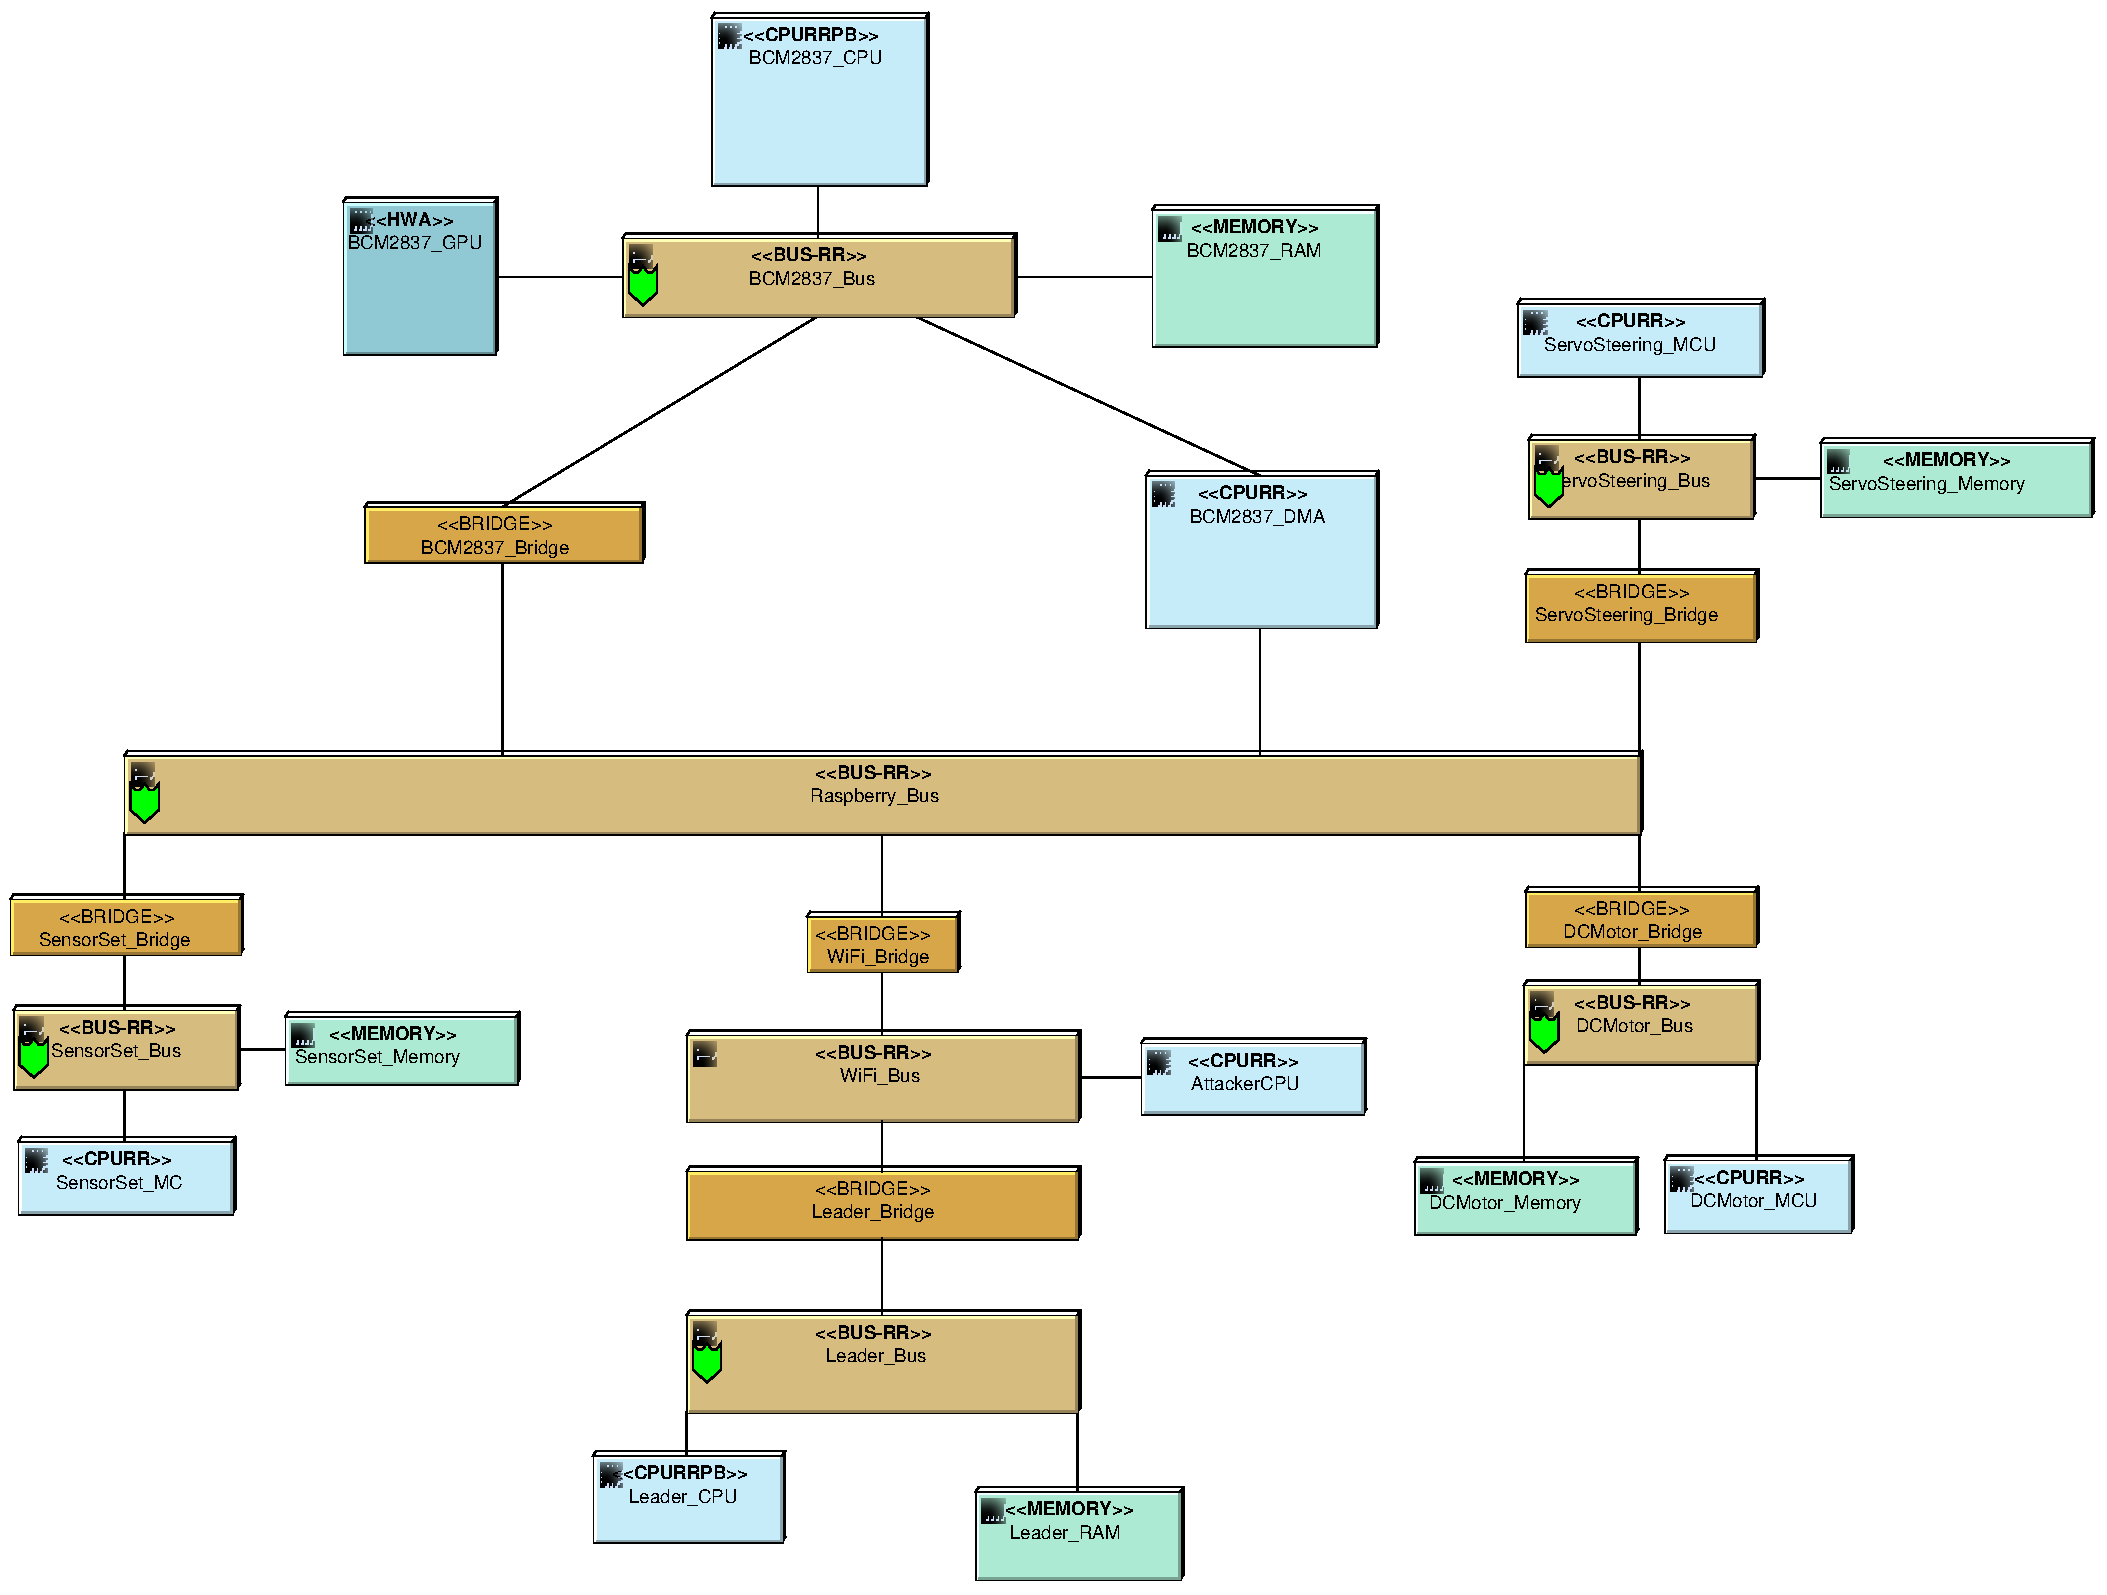
\includegraphics[width=1.2\textwidth]{figures/architecture.pdf}
	\caption{Architecture diagram of the rover}
	\label{fig:roverarchitecture}
\end{figure}

Click now on the \textbf{RoverHardware} tab. You should see the model depicted in Figure~\ref{fig:roverarchitecture}. It represents the hardware platform of the follower: several components are linked to a \texttt{Raspberry\_Bus} modeling the Raspberry Pi board main bus. The set of components prefixed with \texttt{BCM2837} models the Broadcom 2837 SoC acting as the ``core'' of the Raspberry Pi: the driving algorithms will run on the CPU \texttt{BCM2837\_CPU}. On the left, four components are prefixed with \texttt{SensorsSet}: they model the sensors of the rover. Here, we see the sensors as a \{microcontroller, memory\} set: the microcontroller generates the sensors' data, and the memory models a data buffer. You can notice the same modeling strategy for the actuators on the left (components prefixed with \texttt{ServoSteering} and \texttt{DCMotor} respectively).

You will also notice a set of components connected to \texttt{WiFi\_Bus}. These components provide simple models of the leader and the attacker's machine. Indeed, since the leader sends/receives messages to/from the follower we model here, we must model its external logical interfaces (task \texttt{LeaderSocket} in the application model): these interfaces have then to be mapped on hardware component, therefore we need to provide a simple model of the leader. In the same way, the attack tasks that will be added in the application model at W-Sec's next stage must run on hardware components.

\subsubsection{The mapping model}

\begin{figure}
	\centering
	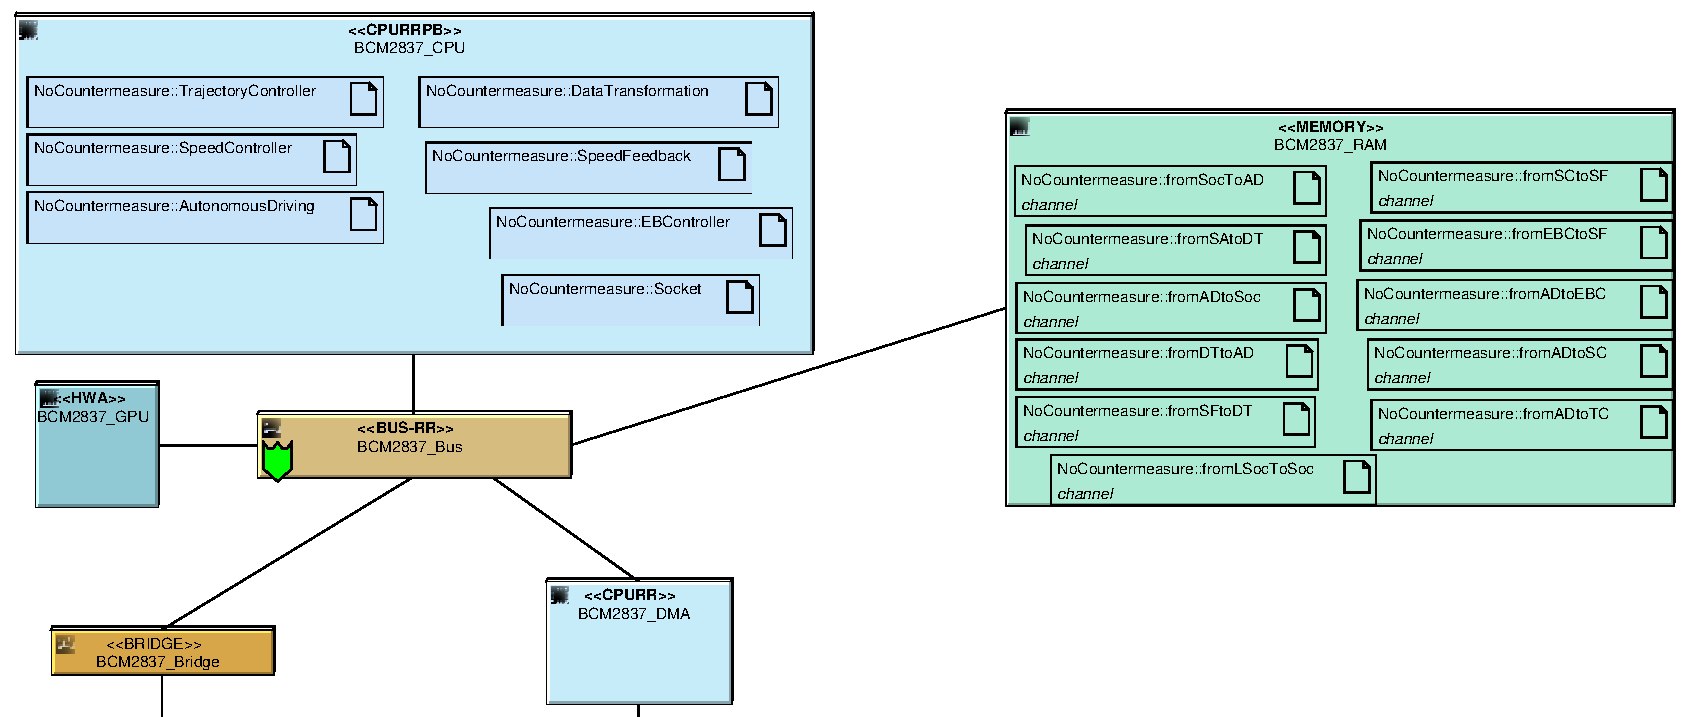
\includegraphics[width=\textwidth]{figures/mapping.pdf}
	\caption{Excerpt of the mapping model}
	\label{fig:rovermapping}
\end{figure}
Open the \textbf{NoCountermeasureMapping} tab. You should now see that all the tasks and the data channels modeled in the \textbf{NoCountermeasure} application model are now allocated to execution nodes (here, CPUs) and memories. Data channels can be mapped on several communication nodes (buses and bridges): for instance, click on the channel \texttt{NoCountermeasure::fromSAtoDT} mapped on \texttt{BCM2837\_RAM} (see figure~\ref{fig:rovermapping}). You should notice red dotted lines: these lines indicate on which communication nodes the channel is mapped, i.e., on which buses and bridges the data conveyed on this channel will transit.

From this mapping view we can now perform model verification (model-checking and simulation).

\subsubsection{The security properties}

As in the AVATAR view for the safety properties, we can directly express the desired security properties in the DIPLODOCUS view. Here, security properties refer to \emph{data} security properties: we can check for each data channel if the data will keep, provided that a Dolev-Yao~\cite{dolevyao} attacker eavesdrops the buses, their:
\begin{enumerate}
	\item confidentiality
	\item integrity (weak authenticity)
	\item integrity and authenticity on origin (strong authenticity).
\end{enumerate}
Open the \textbf{NoCountermeasure} tab and look at the channel \texttt{fromLSocToSoc} between the \texttt{Leader\_Socket} and \texttt{Socket} tasks. You will notice a grey lock: this lock means that the weak and strong authenticity properties for this channel will be checked at the security verification stage. Click now on the port of this channel on the \texttt{Leader\_Socket} task's side. In the dialog box, you can select the option ``Check Confidentiality'': that will also enable the confidentiality verification for this channel at the security verification stage.



%---------------------------------------------------------------------------------------------------------------------------
\section{W-Sec in Practice: creating mutant models}

The second W-Sec stage is a mutation stage, where the models designed in the first stage are enriched with the countermeasure and attack models. In our context, a \emph{model mutation} refers to any modification of a model that leads to another syntactically correct model.

\subsection{AVATAR mutations}

At the end of the first stage, we have $n$ AVATAR models, $n$ being the number of modeled functional scenarios. We denote with $A_i$ this set of models.

For each countermeasure, we first apply a mutation to each element of $A_i$ to enrich it with the countermeasure model. We denote with $A_c$ the resulting set of models. For instance, open \textbf{wsec\_avatar.xml} in TTool. You can notice two tabs named \textbf{MAC} and \textbf{MAC\_Deceleration}. These tabs contain the models of the system enriched with a cryptographic countermeasure, in the context of the two functional scenarios we study. Here, $A_i$ = \{\textbf{Nominal}, \textbf{Nominal\_Deceleration}\} and $A_c$ = \{\textbf{MAC}, \textbf{MAC\_Deceleration}\}. Now, open the \texttt{Rover} library's state machine diagram: you can see that the signal \texttt{inputMessage} now carries a new parameter (\texttt{messageCheck}, modeling the MAC\footnote{\textbf{M}essage \textbf{a}uthentication \textbf{c}ode.}) and that a new state \texttt{FCheckingMAC} has been added. As you can notice, the two transistions that lead to this new state perform a verification of the MAC value: if it is right, the content of the message is taken into account, else, the content of the message is replaced with the content of the last legitimate message the rover has received.

Then for each attack, we apply a mutation to each element of $A_c$ modeling the system in the context of a functional scenario where the attack can occur, to enrich it with the attack model. We denote with $A_{c a}$ the resulting set of models. In our example, the attack can occur in the both functional scenarios. Therefore, you can find in \textbf{wsec\_avatar.xml} two tabs named \textbf{MAC\_Attack1} and \textbf{MAC\_Attack1\_Deceleration}. In our example, $A_{c a}$ = \{\textbf{MAC\_Attack1}, \textbf{MAC\_Attack1\_Deceleration}\}.

In addition, we also apply for each attack a mutation to each element of $A_i$ modeling the system in the context of a functional scenario where the attack can occur, to enrich it with the attack model. We denote with $A_a$ the resulting set of models. As explained above, in our case study the attack can occur in the both functional scenarios. Therefore $A_a$ = \{\textbf{Nominal\_Attack1}, \textbf{Nominal\_Attack1\_Deceleration}\} (see the two tabs in \textbf{wsec\_avatar.xml}). In the \textbf{Nominal\_Attack1} tab, open the state machine diagram of the \texttt{Network} block. You can notice that a new state, named \texttt{interceptingLeaderMessage}, has been added. The transitions leading to this state model the action of the attacker replacing a speed update message with a malicious message containing a higher speed value.


\subsection{DIPLODOCUS mutations}

The DIPLODOCUS models are also enriched with the countermeasure and attack models. At the end of the first W-Sec stage, $n$ DIPLODOCUS models were designed, $n$ being the number of modeled components. We denote with $D_i$ the set of these models. For each countermeasure, we apply a mutation to each element of $D_i$ modeling a component that is targeted by the countermeasure. Then, if needed, we apply to each of these mutant models a new mutation that enriches them with the attack model triggering the countermeasure~\footnote{Indeed, depending on how it is modeled, the countermeasure may need an external ``stimulus'' to be triggered and, therefore, be taken into account in the performance evaluation.}. We denote with $D_{a c}$ the set of these models. In that case, we also apply to each model of $D_i$ mutations that enriches it with the relevant attack(s). We denote with $D_a$ the set of resulting models. For instance, open \textbf{wsec\_diplodocus.xml} in TTool. In our example, $D_a = \{\langle \textbf{NoCountermeasure}, \textbf{NoCountermeasureMapping} \rangle\}$, and $D_{a c} = \{\langle \textbf{MAC}, \textbf{MACMapping} \rangle\}$.

\begin{figure}
	\centering
	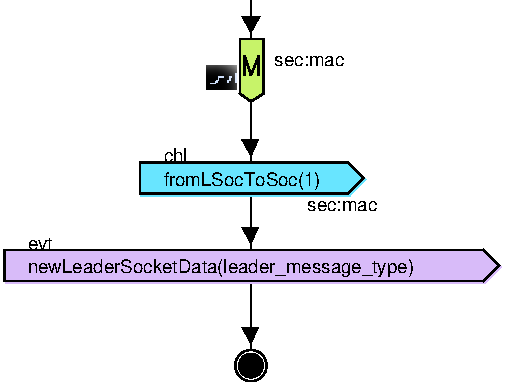
\includegraphics[width=.5\textwidth]{figures/leadersocketmac.pdf}
	\caption{MAC mutation, \texttt{LeaderSocket} task's activity diagram}
	\label{fig:leadersocketmac}
\end{figure}

\begin{figure}
	\centering
	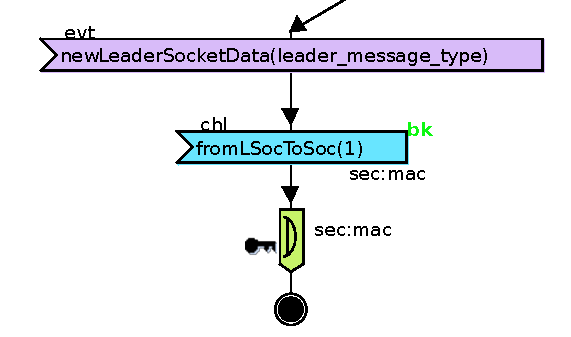
\includegraphics[width=.5\textwidth]{figures/socketmac.pdf}
	\caption{MAC mutation, \texttt{Socket} task's activity diagram}
	\label{fig:socketmac}
\end{figure}

Now, open the \textbf{MAC} tab and then the activity diagram of the \texttt{LeaderSocket} task. You can notice that an encrypt (MAC) operator has been added before the write in channel operator (see Figure~\ref{fig:leadersocketmac}). Open now the \texttt{Socket} task: the corresponding decrypt operator has been added (see Figure~\ref{fig:socketmac}). In the \textbf{MACMapping} tab, you will also notice that a cryptographic key has been mapped to the \texttt{BCM2837\_RAM} and \texttt{Leader\_RAM} memories. The mutation modeling the MAC countermeasure in DIPLODOCUS consists in mapping a key to two memories in the mapping model and in adding two encryption/decryption operators in the application model.


%---------------------------------------------------------------------------------------------------------------------------
\section{W-Sec in Practice: verifying the safety and security properties and performance thresholds}

The third W-Sec stage consists in:
\begin{itemize}
	\item verifying the models designed in stages 1 and 2 against the security and safety properties
	\item simulating the models of $D_a$ and $D_{a c}$ to get performance measurements
	\item comparing these results in order to assess the impacts of the studied countermeasures.
\end{itemize}

\subsection{Verifying the DIPLODOCUS models}

\subsubsection{Security verification}

This stage consists in verifying the models of $D_a$ and $D_{a c}$ against the security properties, and then to compare the model checking results in order to tobserve the security properties each countermeasure enables to recover (positive impact) or makes unreachable (negative impact).

Open \textbf{wsec\_diplodocus.xml} in TTool, and open the \textbf{NoCountermeasureMapping} tab. Perform the syntax analysis, then click on the \textbf{Security verification (ProVerif)} button. Set the \textbf{Compute state reachability} field to \textbf{none}, then click on \textbf{start}. The textbox should provide a \emph{Non Satisfied Authenticity} result for the assessed channel. You can also now click on the \textbf{NoCountermeasure} tab: in the component task diagram, you should notice that the lock linked to the \texttt{fromLSocToSoc} port of the \texttt{Socket} task is red. This backtracing indicates that neither the weak nor the strong authenticity properties are verified on this channel. Click now on the \texttt{MACMapping} tab, and launch the security verification. You should now get a \emph{Satisfied Weak Authenticity} result for the same channel, and the ``W'' part of the lock in the component task diagram under the \textbf{MAC} tab should now be green. This indicates that the channel is protected in integrity (weak authenticity) but not in strong authenticity, since replay attacks can still be led.

Here, the results indicate that the assessed countermeasure provides a net gain with respect to data security.

\subsubsection{Peformance verification}

DIPLODOCUS models can be used to perform another kind of analysis. Indeed, we need to evaluate the performance impact (i.e., the computational overhead) of the countermeasures on the targeted components. This is done thanks to the internal TTool simulator, after the selection of relevant breakpoints that enable, for each component, to measure the time it needs to execute one (or several) loop(s) of its embedded algorithm.

Open the \textbf{NoCountermeasure} tab, and the activity diagram of the \texttt{Socket} task. You can notice that a breakpoint has been placed at the \texttt{fromLSocToSoc} read-in-channel operator. Indeed, we consider that one loop of the driving algorithm of the rover starts at the reception of an update from the leader. Open now the activity diagram of the \texttt{MotorsOutput} task: the second breakpoint has been placed on the \texttt{fromSCtoMO} read-in-channel operator. This message reception indeed occurs each time that a driving control loop ends (the actuators commands have been computed and are now sent to the actuators). Our performance verification here will then measure \textbf{the time the rover needs to compute actuators commands from the moment it receives an update from the leader}.

Now, click on the \textbf{NoCountermeasureMapping} tab and, after performing a syntax analysis, click on the \textbf{Generate code for simulation} button. Generate code, compile, and then launch the simulator. Connect to simulator, and then click on the \textbf{Run simulation} button. The simulator reaches the first breakpoint: it should indicate that 84 cycles and 70 ns were needed. Click again on the \textbf{Run simulation} button: the second breakpoint is reached after 223 cycles and 194 ns. Thus, a loop of the algorithm takes $194 - 70 = 124$ ns. Perform then the same steps for the \textbf{MACMapping} model. You should notice that a loop of the algorithm now takes $1732 - 805 = 927$ ns. This is an important \textbf{relative} variation, but in fact the computational overhead is still acceptable since it is smaller than the rover's sensors acquisition rate (the next iteration of the driving algorithm needs to wait for the next sensors values).

Note that if the performance assessment for a given countermeasure shows that the output of the algorithms could be modified, it may be necessary to perform a new series of mutations on the AVATAR models modeling the system with this countermeasure deployed.


\subsection{Verifying the AVATAR models against the safety properties}

The last verification stage focuses on the system-level safety properties. It aims at providing an assessment of the countermeasures positive (i.e., do they mitigate the attacks from a safety perspective?) and negative (i.e., do they lead to a safety regression?) impacts. To do so, we need to perform safety verification for the models of $A_i$, $A_c$, $A_a$ and $A_{c a}$. The comparison between the results obtained on $A_i$ and $A_a$ will provide the negative impacts (regression) assessment, and the comparison between the results obtained on $A_a$ and $A_{c a}$ will provide the positive impacts (efficiency) assessment.

\subsubsection{Verifying the $A_i$ models}

Open \textbf{wsec\_avatar.xml} in TTool, and go to the \textbf{Nominal} tab. After a syntax analysis, check the two safety pragmas by clicking on the \textbf{Safety verification (Internal tool)} button. Perform the same actions under the \textbf{Nominal\_Deceleration} tab. In the both cases, you should get the following safety verification results:

\cmark~\verb|A[] Environment2.gap > 0|

\cmark~\verb|A[] Environment3.gap > 0|


\subsubsection{Verifying the $A_c$ models}

Perform the safety verification for the \textbf{MAC} and \textbf{MAC\_Deceleration} models. You should obtain the following results:

\cmark~\verb|A[] Environment2.gap > 0|

\cmark~\verb|A[] Environment3.gap > 0|

That means that the MAC countermeasure does not leads to a safety regression with respect to the considered properties.


\subsubsection{Verifying the $A_a$ models}

Now, the safety verification for the \textbf{Nominal\_Attack1} and \textbf{Nominal\_Attack1\_Deceleration} models should provide the following results:

\xmark~\verb|A[] Environment2.gap > 0|

\xmark~\verb|A[] Environment3.gap > 0|

In other terms, on the initial system, the attack leads to a regression for both considered safety properties.

\subsubsection{Verifying the $A_{c a}$ models}

You can now launch the safety verification for the \textbf{MAC\_Attack1} model. You should obtain these results:

\cmark~\verb|A[] Environment2.gap > 0|

\cmark~\verb|A[] Environment3.gap > 0|

In the first functional scenario, the MAC countermeasure thus enables the mitigation of the attack. Now, perform the verification for \textbf{MAC\_Attack1\_Deceleration}. The verifyer gives the following results:

\xmark~\verb|A[] Environment2.gap > 0|

\xmark~\verb|A[] Environment3.gap > 0|

The countermeasure can't avoid a crash of the swarm if the leader decelerates when an attack occurs.\\

At the end of this third W-Sec stage, an assessment of the countermeasures with respect to safety, security and performance aspects are thus provided. In this tutorial we evaluate only one countermeasure and one attack scenario: if you want to see how the method can help ranking countermeasures on the basis of exhaustive results, the paper introducing W-Sec~\cite{wsec} provides a full analysis of five countermeasures, four attack scenarios and four functional scenarios on this rover swarm case-study.



%---------------------------------------------------------------------------------------------------------------------------
\section{W-Sec in Practice: enriching the initial model set}

Depending on the countermeasure(s) that is(are) chosen to be deployed at the end of a W-Sec iteration, the model set defined at the first stage may need to be updated in order to keep it representative to the system. For instance, if we decide to deploy the MAC countermeasure, the models \textbf{Nominal} and \textbf{Nominal\_Deceleration} shall be replaced with \textbf{MAC} and \textbf{MAC\_Deceleration} that are now the nominal models of the system.



%---------------------------------------------------------------------------------------------------------------------------
\section{Conclusion}

This document provides a tutorial on W-Sec, a TTool-based formal method dedicated to provide a comprehensive impact assessment of security countermeasures. The practical aspects of the method are meant to evolve: the stage 2 and part of the stage 1, that currently require a full human intervention, will be automated in the future.



\bibliographystyle{acm}
\bibliography{biblio}

\end{document}
